\chapter{Аналитическая часть}

В данной части будут описаны алгоритмы.

\section{Формализация объектов синтезируемой сцены}

Объекты сцены:
\begin{enumerate}
	\item ландшафт -- поверхность задаваемая картой высот. Может быть задана как с помощью заранее предопределённых значений, так и методом случайной генерации;
	\item источник света -- точка в пространстве освещающая сцену в заданном направлении. Характеризуется цветом и интенсивностью;
	\item камера -- объект который задаёт направление взгляда наблюдателя, характеризуется вектором. 
\end{enumerate}

\section{Методы описания поверхностей}

\subsection{Аналитическая модель}

Данная модель подразумевает формальное описание математическими формулами. Обычно такая модель может быть описана функцией от двух переменных~(\ref{eq:analit_1}).

\begin{equation}
	z = f(x, y)
	\label{eq:analit_1}
\end{equation}

Или может быть описана формулой~(\ref{eq:analit_2}).

\begin{equation}
	F(x, y, z) = 0
	\label{eq:analit_2}
\end{equation}

Зачастую для описания таких поверхностей используются кусочно заданные функции, например сплайны. Сплайн -- это кусочно заданная функция пригодная для аппроксимации отдельных фрагментов поверхности. 

Преимущества данного подхода:
\begin{itemize}
	\item не большой объём занимаемой памяти;
	\item простой расчёт положения каждой точки модели.
\end{itemize}

Недостатки:
\begin{itemize}
	\item расчёт по аналитическим формулам может занимать много времени;
	\item не для всякой поверхности удобно использовать данный подход или вовсе возможно;
\end{itemize}

\subsection{Воксельная модель}

Воксельная модель~\cite{voxel} является трёхмерным растром. Подобно пикселям которые располагаются на плоскости, воксели располагаются в некотором объёме.

Преимущества данной модели:
\begin{itemize}
	\item простота описания сложных объектов;
	\item простота преобразований;
	\item простота отображения на экран.
\end{itemize}

Недостатки:
\begin{itemize}
	\item большой объём требуемой памяти;
	\item проблемы с точностью модели;
	\item небольшая скорость обработки.
\end{itemize}

\subsection{Неравномерная сетка}

Равномерной сеткой назовём множество заданных точек вида: $\{(x_0, y_0, z_0) \dots (x_n, y_n, z_n)\}$, которые принадлежат поверхности. 

Преимущества данной модели:
\begin{itemize}
	\item можно использовать только важные опорные точки, что ведёт к уменьшению объёма требуемой памяти.
\end{itemize}

Недостатки:
\begin{itemize}
	\item могут возникать проблемы при масштабировании изображения.
\end{itemize}

\subsection{Равномерная сетка}

Способ задания модели с помощью равномерной сетки отображён на рисунке~\ref{fig:r_setka}.

\begin{figure}[H]
	\centering
	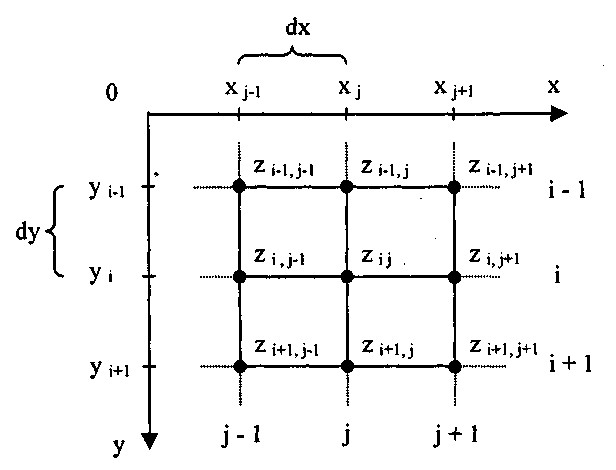
\includegraphics[height=0.35\textheight]{ravn_setka.png}
	\caption{Представление высот с помощью равномерной сетки}
	\label{fig:r_setka}
\end{figure}

Каждый узел с индексами $i, j$ равномерной сетки содержит высоту $Z_{ij}$. По сути мы получаем однозначную формулу~(\ref{eq:rs}) для получения высоты $Z$.

\begin{equation}
	Z = f(i, j)
	\label{eq:rs}
\end{equation}

Преимущества данной модели:

\begin{itemize}
	\item простота представления сложных моделей;
	\item быстрота обработки модели;
	\item возможность получить значения любой точки с помощью интерполяции.
\end{itemize}

Недостатки:
\begin{itemize}
	\item равномерная сетка может быть представлена как однозначная формула~(\ref{eq:rs}), это обозначает невозможность задания поверхностей которые соответствуют неоднозначным функциям;
	\item невозможность задания вертикальных граней.
\end{itemize}

\subsection*{Выбор метода описания поверхности}

Для решения поставленной задачи был выбран метод представления ландшафта в виде равномерной сетки. Ограничения этого метода, связанные с однозначностью функции z = f(x, y) и невозможностью моделирования вертикальных граней, являются незначительными и вполне приемлемыми. Метод регулярной сетки обеспечивает простоту описания поверхности и часто используется для моделирования рельефа земной поверхности.

\section{Алгоритмы построения карты высот}

\subsection{Задание высот случайными числами}

Данный метод задаёт каждую точку карты высот случайным числом.

Преимущества данного алгоритма:

\begin{itemize}
	\item простая реализация.
\end{itemize}

Недостатки:

\begin{itemize}
	\item невозможность построения реалистичного ландшафта;
	\item слабый контроль.
\end{itemize}

\subsection{Холмовой алгоритм}
В данном методе все точки карты высот изначально находятся на одном уровне. Затем случайным образом вносятся холмы с случайно заданным радиусом.

Преимущества данного алгоритма:

\begin{itemize}
	\item возможность получения реалистичного ландшафта.
\end{itemize}

Недостатки:

\begin{itemize}
	\item нереалистичность ландшафта при малом количестве итераций;
	\item необходимость различных оптимизаций алгоритма для достижения реалистичного ландшафта.
\end{itemize}

\subsection{Построение карты высот с помощью диаграммы Вороного}

Диаграмма вороного~\cite{voronoi} – это разбиение плоскости на n областей, в виде выпуклых многоугольников для n точек. Каждая область содержит в себе только одну точку. Имеется четыре алгоритма постройки диаграммы и самым быстрым и известным является алгоритм Форчуна. Пример диаграммы изображён на рисунке~\ref{fig:voron}.


\begin{figure}[H]
	\centering
	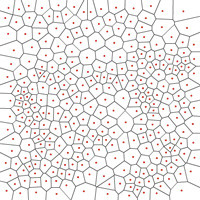
\includegraphics[height=0.3\textheight]{voron.png}
	\caption{Диаграмма Вороного построенная с помощью алгоритма Форчуна}
	\label{fig:voron}
\end{figure}

\subsection{Алгоритм diamond-square}

Данный алгоритм~\cite{diamond_square} работает с равномерной сеткой. Он является расширением алгоритма <<midpoint displacement>> который работает с отрезком. Суть алгоритма заключается в внесении случайного смещения по центру отрезка, затем отрезок рабивается на две равные части, после чего алгоритм рекурсивно повторяется для этих половинок. Причём на каждой итерации алгоритма максимальное значение смещения по модулю уменьшается. Пример работы этого алгоритма изображён на рисунке~\ref{fig:mid_dis}

\begin{figure}[H]
	\centering
	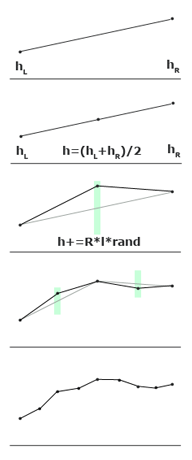
\includegraphics[height=0.3\textheight]{mid_dis.png}
	\caption{Пример работы алгоритма midpoint displacement}
	\label{fig:mid_dis}
\end{figure}
 
Этот алгоритм можно обобщить и для плоскости, работать он будет следующим образом: плоскость разбивается на четыре равных квадрата, значение в углах квадратов получаются путём интерполяции и добавлением случайного смещения.

Алгоритм <<diamond-square>> отличается от двумерного <<midpoint displacement>>, тем что он состоит из двух этапов:

\begin{enumerate}
	\item <<square>> -- определяет точку посередине квадрата путём интерполяции высот угловых точек и добавления смещения;
	\item <<diamond>> -- определяет высоту точек лежащих на серединах сторон квадратов, путём интерполяции значений концов стороны и двух середин смежных квадратов.
\end{enumerate}

Пример работы данного алгоритма изображён на рисунке~\ref{fig:diamond_square}.

\begin{figure}[H]
	\centering
	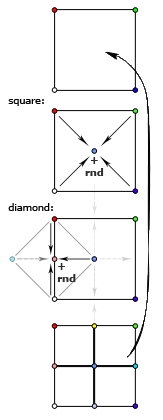
\includegraphics[height=0.3\textheight]{diamond_square.png}
	\caption{Пример работы алгоритма diamond-square}
	\label{fig:diamond_square}
\end{figure}

Преимущества данного алгоритма:
\begin{itemize}
	\item получение крайне реалистичного ландшафта;
	\item простота реализации.
\end{itemize}

Недостатки:

\begin{itemize}
	\item шум при больших картах.
\end{itemize}

\subsection*{Выбор алгоритма построения карты высот}

Поскольку для представления ландшафта используется равномерная сетка высот, предпочтительным алгоритмом является алгоритм <<diamond-square>>. Этот алгоритм также позволяет гибко настраивать параметры, что дает возможность получать разнообразные и одновременно очень реалистичные ландшафты.

\section{Алгоритмы удаления невидимых линий и поверхностей}

\subsection{Алгоритм Варнока}

Алгоритм работает в пространстве изображения. Производится разбиение области на <<окна>>. Для каждого из них решается вопрос о том, пусто ли «окно», либо его содержимое «достаточно просто» для визуализации. Если это не так, то окно рекурсивно разбивается на фрагменты до тех пор, пока содержимое не станет «достаточно простым» для визуализации. В случае достижения минимального предела размера полученного окна необходимо вычислить глубину каждого элемента его содержимого и визуализировать тот из них, который расположен ближе остальных к точке наблюдения. 

Преимущества данного алгоритма:

\begin{itemize}
	\item при увеличении размеров однородных областей изображения повышается скорость работы.
\end{itemize}

Недостатки:

\begin{itemize}
	\item в сложных сценах количество разбиений может стать чрезмерно большим. 
\end{itemize}

\subsection{Алгоритм Робертса}

Данный алгоритм работает в объектном пространстве. Сначала для каждого объекта удаляются грани которые скрываются самим объектом. Затем каждое из видимых ребер каждого тела сравнивается с каждым из оставшихся тел для определения частей, скрывающихся этими телами.

Преимущества данного алгоритма:

\begin{itemize}
	\item высокая точность;
	\item низкая сложность математических операций.
\end{itemize}

Недостатки:

\begin{itemize}
	\item значительное замедление при увеличении объектов сцены.
\end{itemize}

\subsection{Алгоритм трассировки лучей}

В этом алгоритме для каждого пикселя изображения выпускается луч, который пересекает грани объектов. Для визуализации выбирается ближайшее пересечение.

Преимущества данного алгоритма:

\begin{itemize}
	\item реалистичность отображаемых гладких объектов без их аппроксимации примитивами;
	\item линейная зависимость вычислительной сложности от количества элементов на сцене. 
\end{itemize}

Недостатки:

\begin{itemize}
	\item требуется большое количество вычислений, в особенности при высоком разрешении создаваемого изображения. 
\end{itemize}

\subsection{Алгоритм, использующий Z-буфер}

Алгоритм~\cite{z_buf} функционирует в пространстве изображения и использует буфер кадра для хранения интенсивности каждого пикселя. Он также сохраняет глубину каждого пикселя в Z-буфере. При добавлении нового пикселя в буфер кадра его значение глубины сравнивается с глубиной уже сохраненного пикселя в Z-буфере. Если глубина нового пикселя меньше, он заменяет ранее сохраненный пиксель, и Z-буфер обновляется. Если же глубина нового пикселя больше, никаких действий не требуется.

Преимущества данного алгоритма:

\begin{itemize}
	\item простота релизации;
	\item отсутствие необходимости сортировки элементов сцены.  
\end{itemize}

Недостатки:

\begin{itemize}
	\item увеличение затрат памяти на хранение дополнительной информации о глубине отображемых пикселов.
\end{itemize}

\subsection*{Выбор алгоритма удаления невидимых линий и поверхностей}

Наиболее подходящим для решения поставленной задачи выбран алгоритм, использующий Z-буфер, поскольку он прост в реализации, обеспечивает достаточно реалистичное изображение для данной задачи и не требует значительных вычислительных ресурсов, в отличие от алгоритмов, которые могут обеспечить более высокую степень реалистичности изображения.

\section{Модели освещения}

Модели освещения можно поделить на локальные и глобальные. Глобальные модели учитывают преломление и отражение света от объектов, локальные учитывают исключительно освещение самих источников. 

Освещение объектов складывается из трёх составляющих:

\begin{enumerate}
	\item фоновая -- константа окружающего освещения, которая всегда будет придавать объекту некоторый оттенок; 
	\item диффузная -- имитирует воздействие на объект направленного источника света; 
	\item зеркальная — имитирует блик света, который появляется на блестящих объектах. 
\end{enumerate}

\subsection{Модель освещения Ламберта}

Эта модель позволяет реализовать диффузное освещение объектов, при котором свет, попадая на поверхность, рассеивается равномерно во всех направлениях. При расчете такого освещения учитываются только ориентация поверхности и направление на источник света. Интенсивность отраженного света не зависит от положения наблюдателя. Цвет, который мы видим на матовой поверхности, определяется комбинацией ее собственного цвета и цвета света, исходящего от источника. Интенсивность отражения пропорциональна косинусу угла между внешней нормалью к поверхности и направлением на источник света.

\subsection{Модель освещения Фонга}

Эта модель позволяет сочетать диффузную и зеркальную составляющие, что дает возможность появления бликов на материале. Падающий и отраженный лучи находятся в одной плоскости с нормалью к отражающей поверхности в точке падения, и эта нормаль делит угол между лучами на две равные части. Интенсивность отраженной освещенности в данной точке зависит от того, насколько близки направления вектора, направленного на наблюдателя, и отраженного луча.

\subsection{Выбор модели освещения}

Объекты создаваемой сцены не требуют зеркального отражения и рассматриваются как матовые. В связи с этим целесообразно использовать локальную модель освещения без зеркальной составляющей. Создание бликов отраженного света не является необходимым для данной задачи. Учитывая эти факторы, оптимальной моделью освещения будет модель Ламберта.

\section{Алгоритмы закраски}

\subsection{Простой алгоритм закраски}

При применении данного алгоритма окраска всей поверхности имеет одинаковый уровень интенсивности, и для вычислений используется закон Ламберта. Алгоритм обеспечивает высокое качество изображений только в том случае, если источник света и наблюдатель находятся на значительном расстоянии от объекта, а каждая грань тела не является аппроксимирующей поверхностью.

Преимущества данного алгоритма:

\begin{itemize}
	\item простота реализации;
	\item быстродействие
\end{itemize}

Недостатки:

\begin{itemize}
	\item видимые переходы между гранями у аппроксимированных гладких объектов;
	\item низкая правдоподобность изображения зеркальных бликов.
	
\end{itemize}

\subsection{Закраска Гуро}

Алгоритм закраски Гуро основан на интерполяции интенсивности и позволяет получать качественные изображения гладких поверхностей. Суть метода заключается в том, что освещение не усредняется для всей грани, а линейно интерполируется между вершинами. В этой модели нормали задаются в вершинах.

Преимущества данного алгоритма:

\begin{itemize}
	\item достаточно качественное отображение гладких поверхностей;
\end{itemize}

Недостатки:

\begin{itemize}
	\item появление полос Маха;
	\item низкая правдоподобность изображения зеркальных бликов.
\end{itemize}

\subsection{Закраска Фонга}

 Алгоритм закраски Фонга основан на интерполяции вектора нормали.  Цвет, в свою очередь, рассчитывается для каждого пикселя в отдельности.  
 
 Преимущества данного алгоритма:
 
 \begin{itemize}
 	\item высокая правдоподобность изображения зеркальных бликов;
 	\item достаточно качественное отображение гладких поверхностей.
 \end{itemize}
 
 Недостатки:
 
 \begin{itemize}
 	\item требуется большое количество вычислительных ресурсов.
 \end{itemize}


\subsection*{Выбор алгоритма закраски}

Для демонстрации алгоритма генерации ландшафтных поверхностей не обязательно добиваться высокой реалистичности цветового отображения. В данном случае предпочтительнее использовать максимально эффективный алгоритм, а именно – плоскую закраску, поскольку значительное время обработки будет затрачено на трехмерные преобразования сцены, требующие длительных тригонометрических вычислений.

\section*{Вывод}

В этом разделе были рассмотрены методы создания реалистичных изображений. Описаны характеристики объектов сцены и способы их представления, а также проанализированы различные алгоритмы рендеринга и модели освещения. На основе проведенного анализа был сделан выбор в пользу равномерной сетки, модели освещения Ламберта и алгоритма использующего Z буфер. Эти методы являются наиболее подходящими для разработки алгоритма, способного реалистично отображать реалистичный ландшафт.

